\documentclass[a4paper,12pt]{jarticle}
\input ./chap01_preamble.tex
\graphicspath{%
  {../text01-img/}%
}
% !TEX root = ./chap01_01.tex
\begin{document}
\section{今回の授業}
\subsection{目標}
\ \ \ \ ラズベリーパイになれよう

\ \ \ \ 自分のホームページを作れるようになろう

\subsection{授業内容}
%\liststyleLii
\begin{enumerate}
  \item ラズベリーパイとは
  \item ラズベリーパイになれよう(1)
  \item ラズベリーパイになれよう(2)
  \item 自分の紹介ページを作ろう
\end{enumerate}
\subsection{注意点}
%\liststyleLiii
\begin{itemize}
  \item
        授業の合間のきゅうけいでは、遠くのものをながめたりして目を休めましょう
  \item 水分ほきゅうはこまめにしましょう
  \item
        先生が説明中は先生の話を聞きましょう
  \item
        わからないことがあったらTAの先生方にすぐ聞きましょう
\end{itemize}
\subsection{教科書について}
%\liststyleLiv
\begin{itemize}
  \item
        教科書には例題、それに似た問題があります。まずは、例題をよく読みながら試してみましょう。そのあと問題を解きましょう。問題の答えは一番最後のページにあります。
\end{itemize}
\clearpage\subsection{配布物の確認}

\bigskip

%\liststyleLv
\begin{enumerate}
  \item ラズベリーパイ
  \item SDカード(16GB)
  \item でんげんケーブル
  \item HDMIケーブル
  \item GPIOエクステンダー
  \item ヘッドセット
  \item マウス
  \item センサーボード
  \item ウェブカメラ
  \item ディスプレイ(持って帰れません)
\end{enumerate}
\clearpage

\begin{tabular}{cc}
  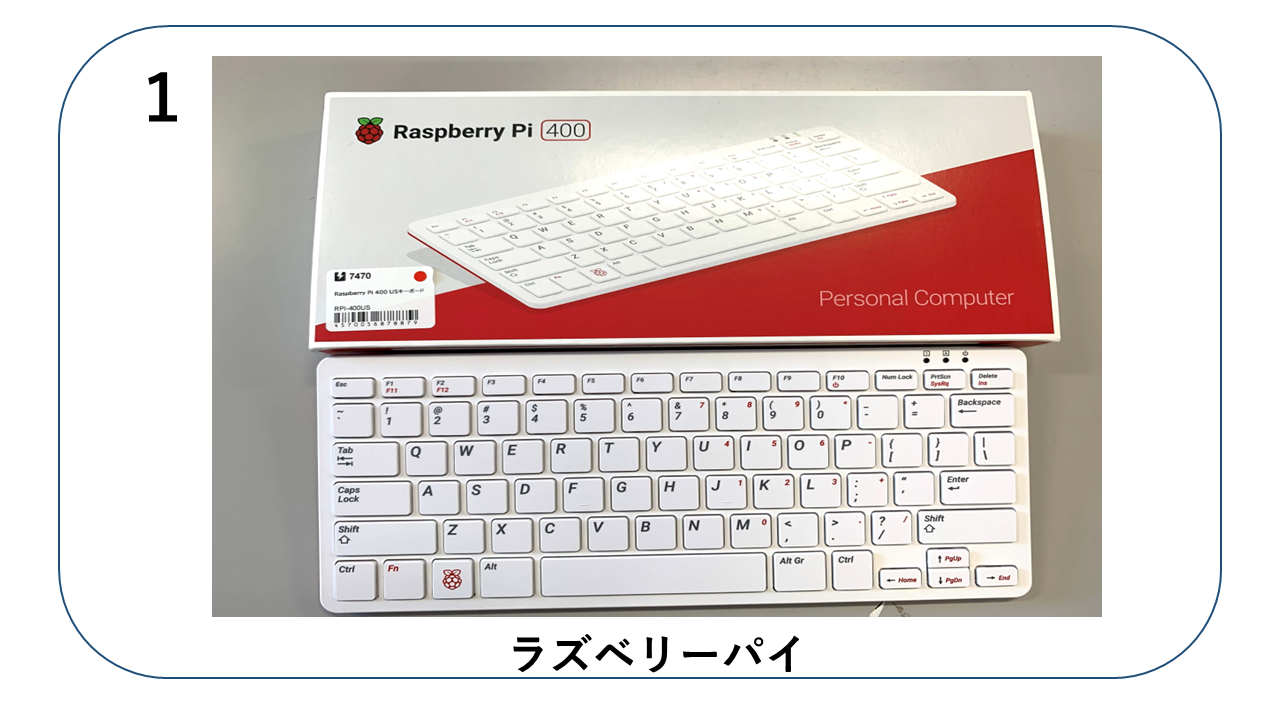
\includegraphics[width=6.488cm,height=4.697cm]{textbook-img009-2023.png}
   &
  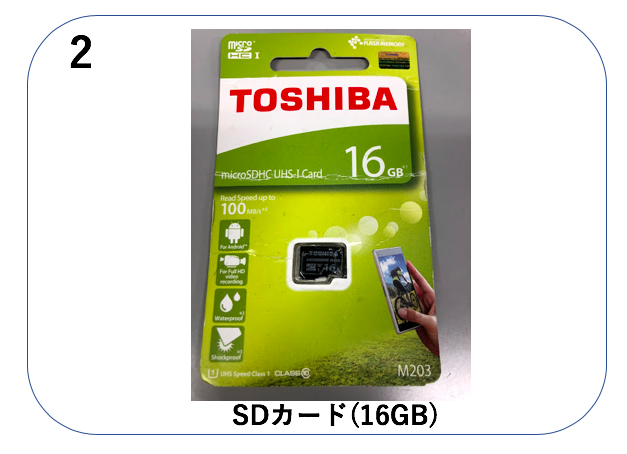
\includegraphics[width=6.488cm,height=4.697cm]{textbook-img010.png} \\

  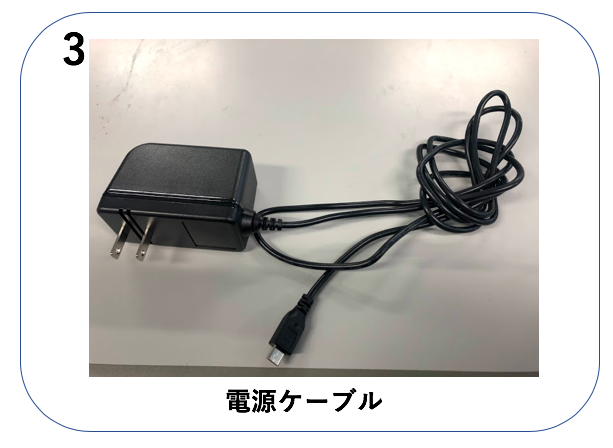
\includegraphics[width=6.488cm,height=4.697cm]{textbook-img007.png}
   &
  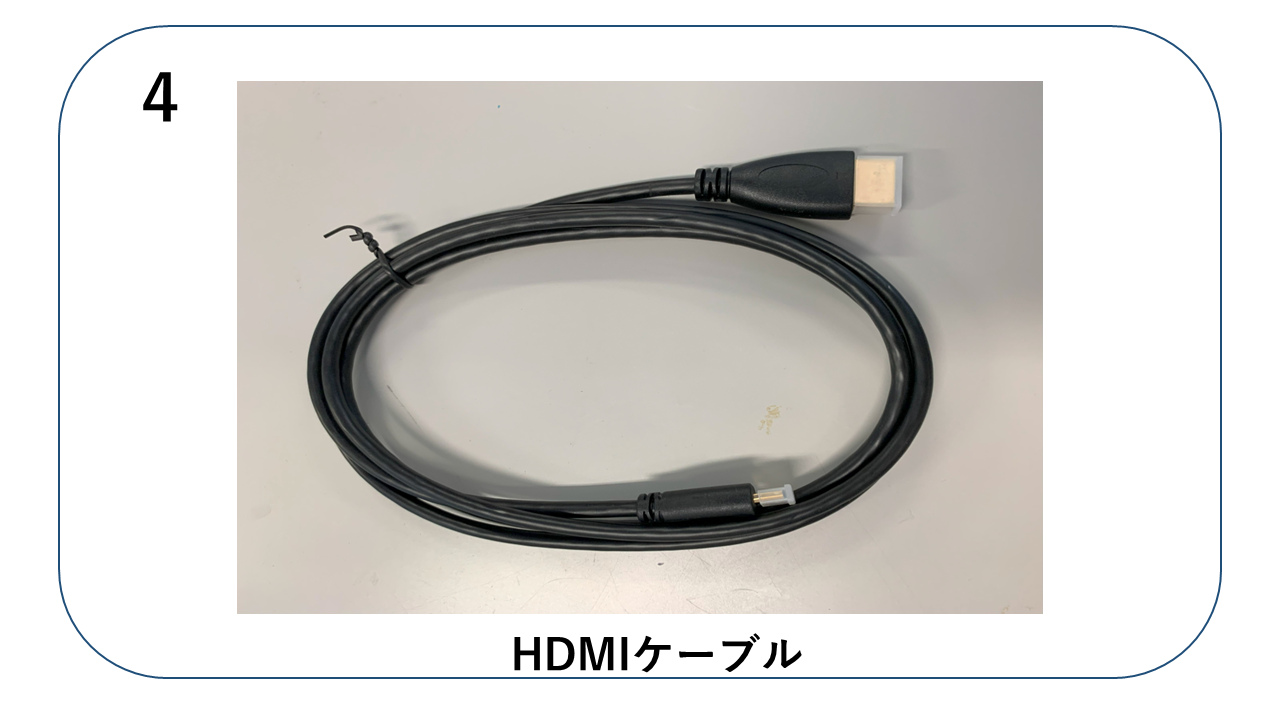
\includegraphics[width=6.488cm,height=4.697cm]{textbook-img008-2023.png} \\

  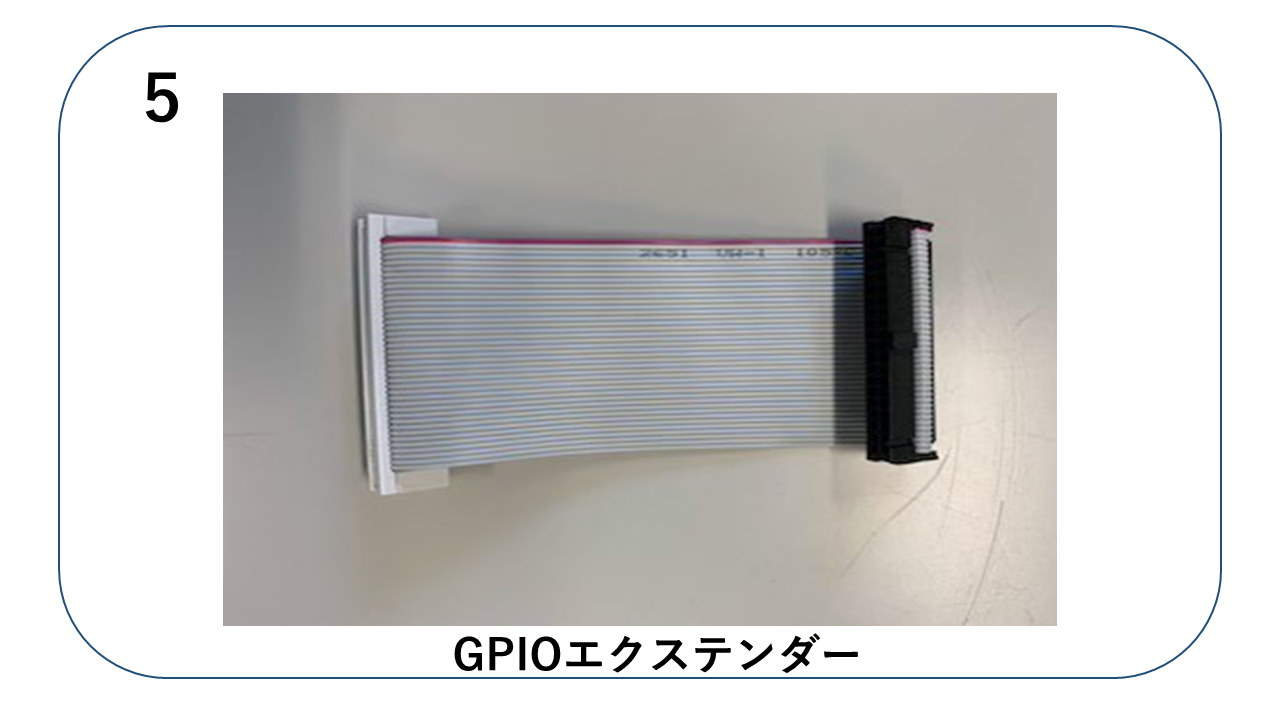
\includegraphics[width=6.488cm,height=4.697cm]{textbook-img005-2023.png}
   &
  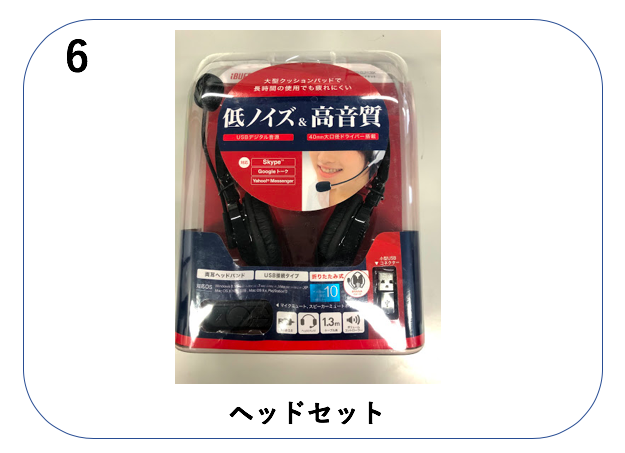
\includegraphics[width=6.488cm,height=4.697cm]{textbook-img006.png} \\

  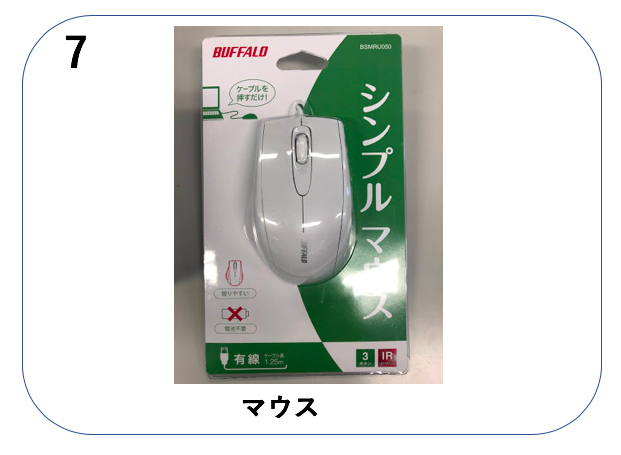
\includegraphics[width=6.488cm,height=4.697cm]{textbook-img003.png}
   &
  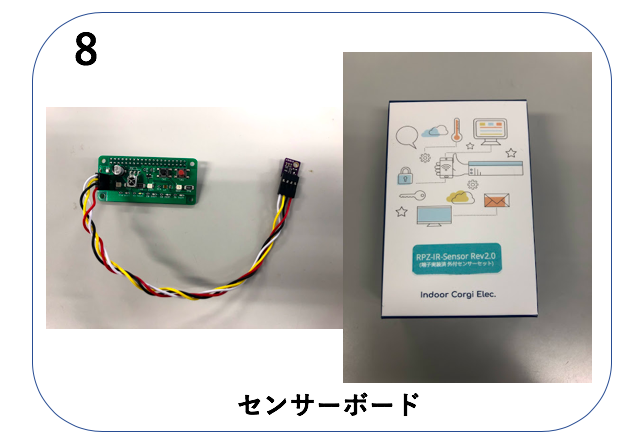
\includegraphics[width=6.488cm,height=4.697cm]{textbook-img004.png} \\

  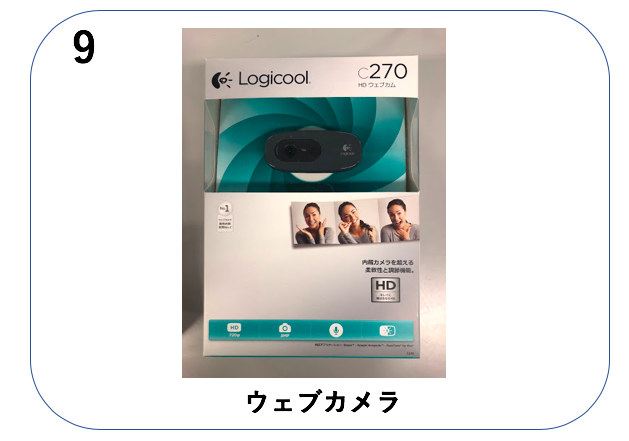
\includegraphics[width=6.488cm,height=4.697cm]{textbook-img002.png}
   &
  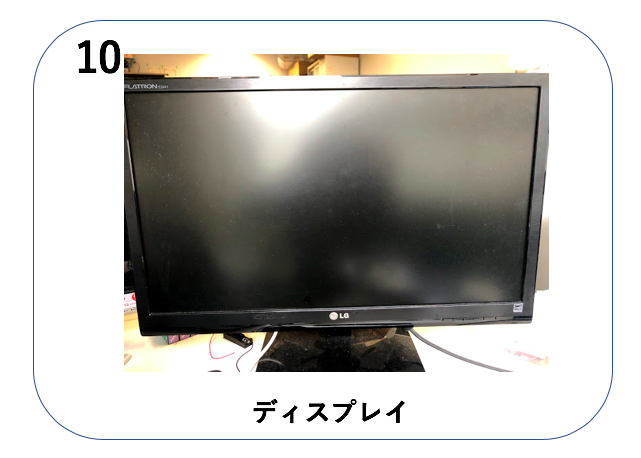
\includegraphics[width=6.488cm,height=4.697cm]{textbook-img001.png} \\
\end{tabular}

%\liststyleLv
\subsection{ラズベリーパイについて}
イギリスのラズベリーパイ財団というグループが開発したキーボード一体型のコンピュータです。ラズベリーパイは短くラズパイとも呼ばれています。

\subsection{とくちょう}
%\liststyleLvi
\begin{itemize}
  \item キーボード一体型で、キーボードが必要ない
  \item 普通のパソコンのように使える
  \item (動画再生やゲームもできます)
  \item
        プログラミングのべんきょうに向いている
  \item
        モータやライトをせいぎょできる(目に見えるのでプログラミングを楽しめる)
\end{itemize}
\subsection{ラズベリーパイでできること}
プログラミングを手軽に学ぶことができます。プログラミングをするときにはパソコンが必要

でお金もかかりやりたくてもできないひともいたかもしれません。しかし、ラズベリーパイの

ような小さくて手に入れやすいコンピュータがあれば手軽にプログラミングの学習に取り組む

ことができます。また、ラズベリーパイを使うことでモータやライトなどを動かしたり光らせ

たりすることができます。これらのせいぎょをプログラムで行うことができるので楽しみなが

ら学習を進められます。

\subsection{ラズベリーパイを使うときの注意}
%\liststyleLvii
\begin{itemize}
  \item
        水などぬれているものをラズベリーパイ本体につけないようにしましょう
\end{itemize}
%\liststyleLviii
\begin{itemize}
  \item
        ラズベリーパイをはじめコンピュータなどは熱に弱いのですごく暑い部屋では使わないようにしましょう
\end{itemize}
%\liststyleLix
\begin{itemize}
  \item
        ラズベリーパイの本体をあまりさわらないようにしましょう
  \item
        ラズベリーパイなどは静電気によわいので注意しましょう
\end{itemize}
%\liststyleLx
\begin{itemize}
  \item
        ラズベリーパイをらんぼうに扱うのはやめましょう
\end{itemize}
%\liststyleLxi
\begin{itemize}
  \item
        金属のものの上におかないようにしましょう
\end{itemize}

\clearpage

\subsection{ラズベリーパイを準備しよう(手順)}
\ \ ラズベリーパイとキーボード、マウス等を接続して起動する準備をします。

\begin{figure}[ht]
  \centering
  \begin{minipage}{12.204cm}
    {\upshape
      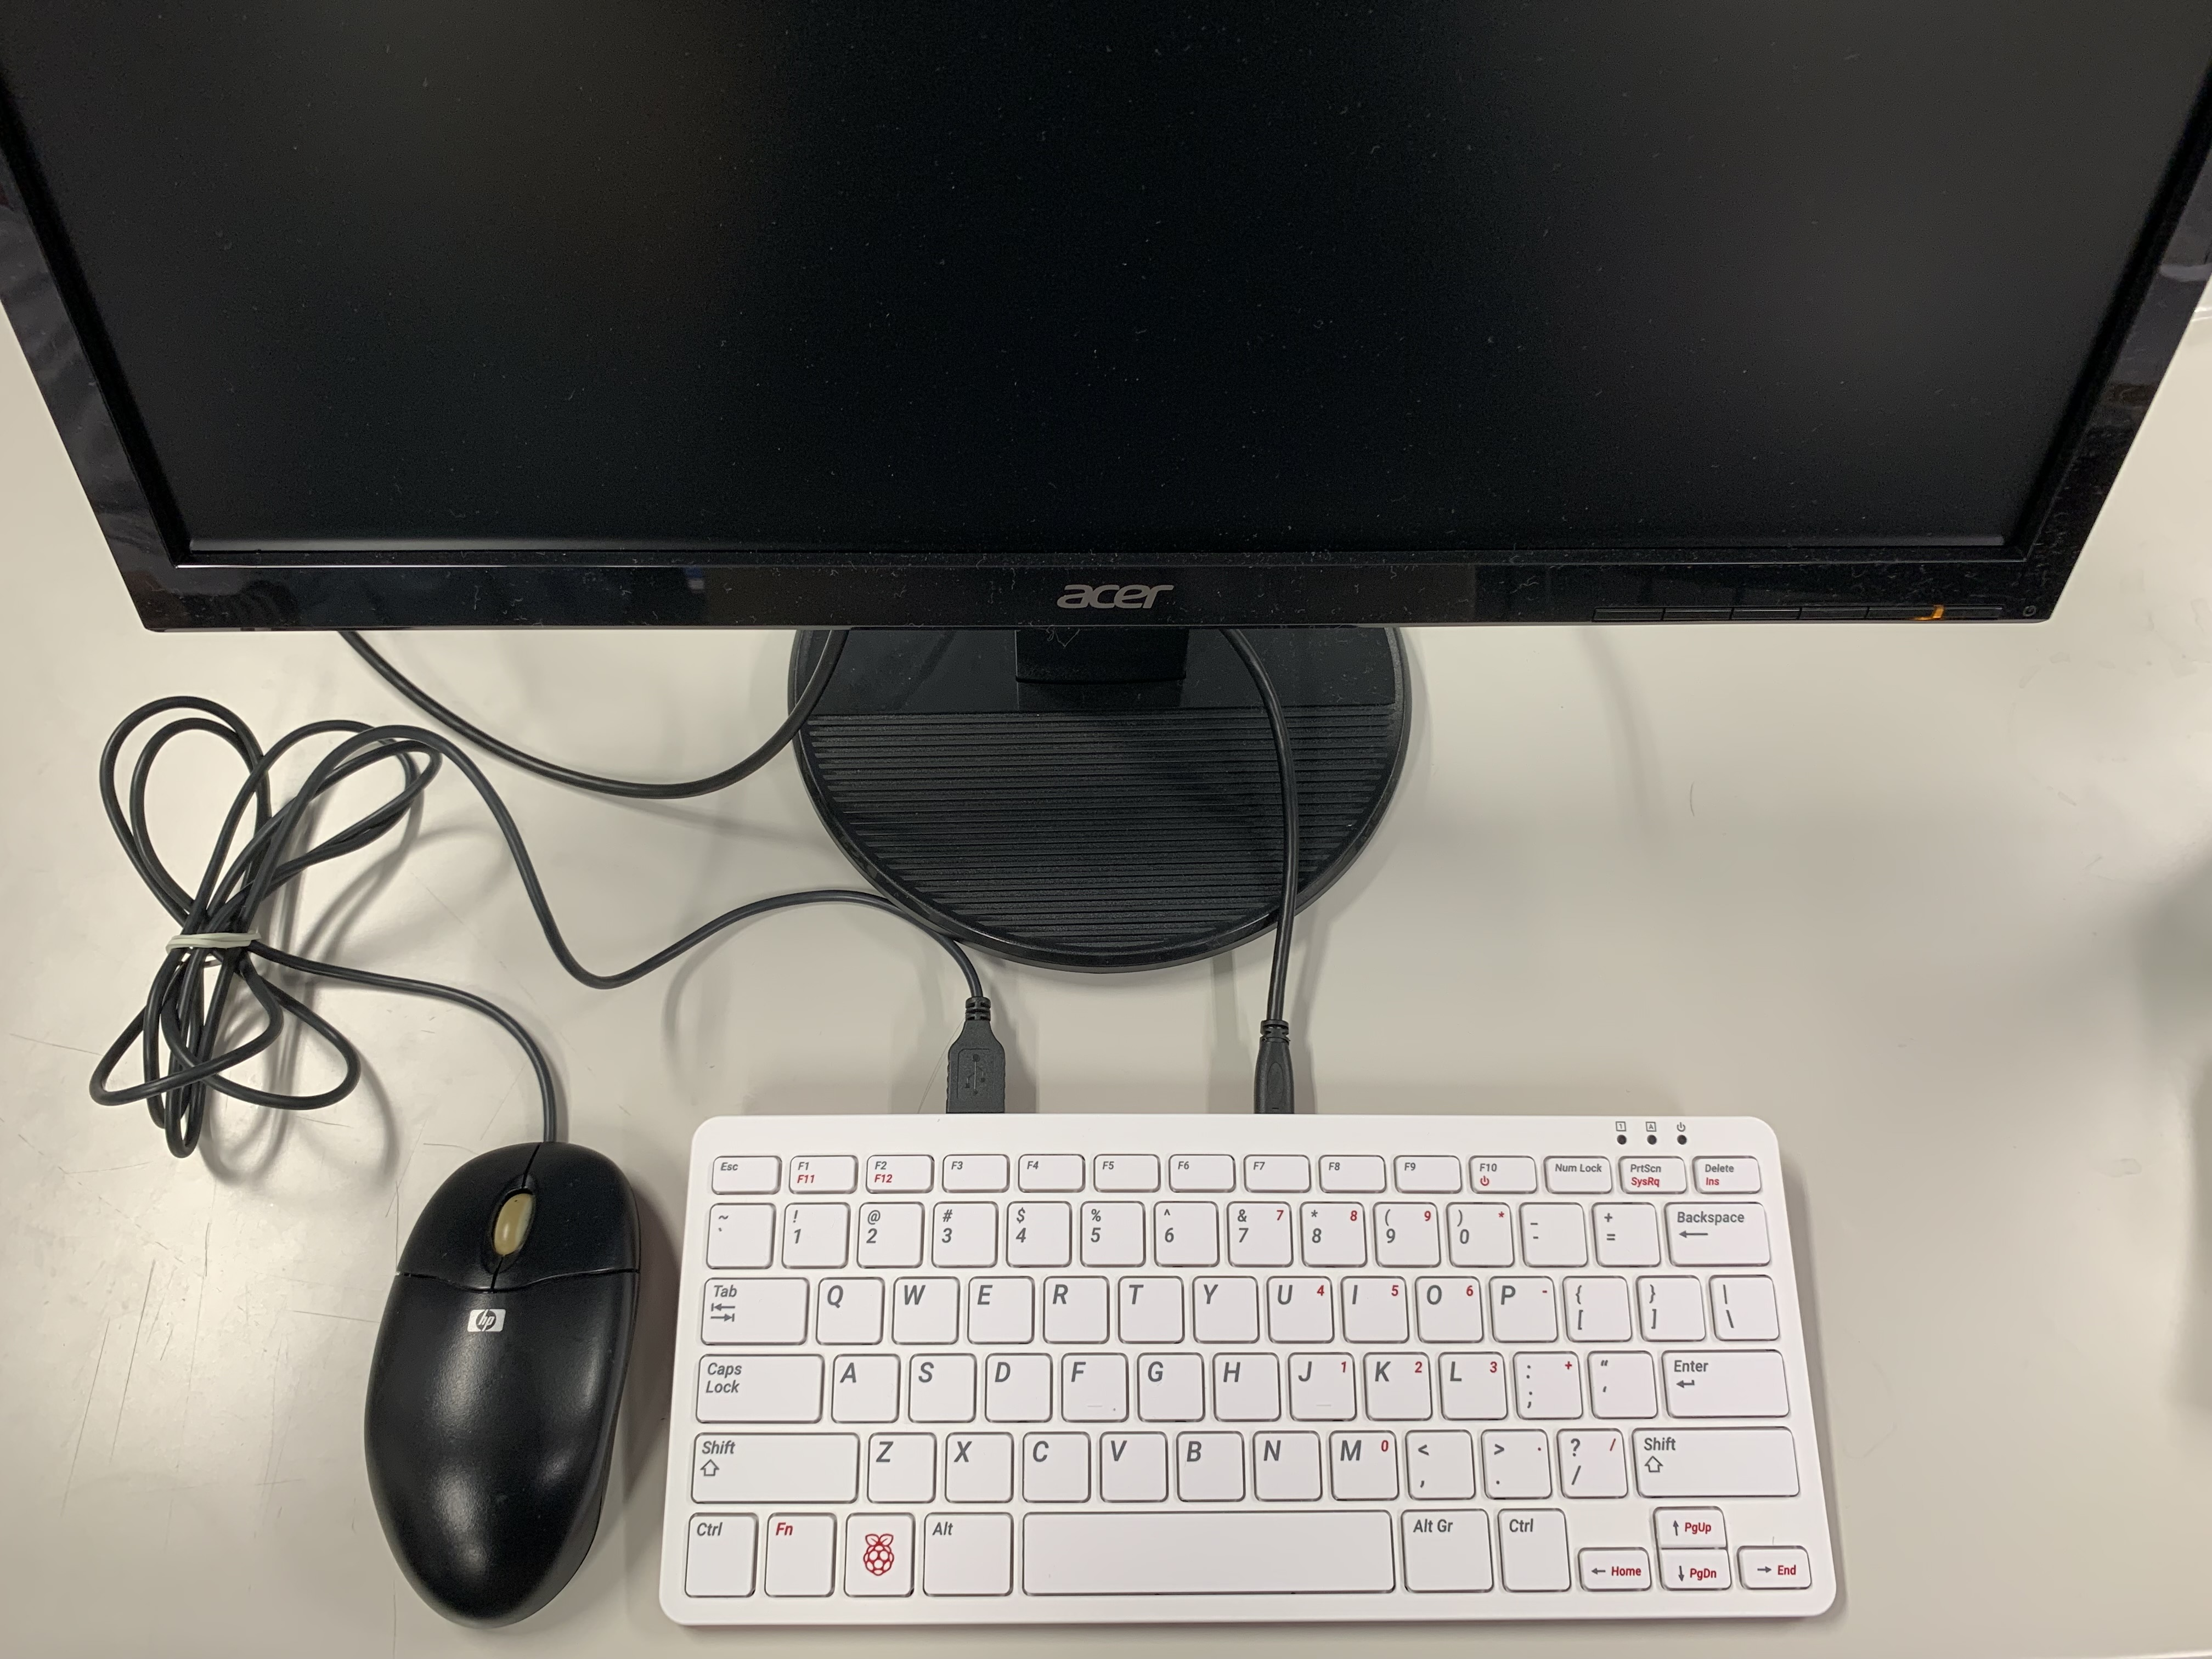
\includegraphics[width=0.6\textwidth]{connections01-2023.jpg}
      \newline
      Figure \stepcounter{Figure}{\theFigure}: 接続の全体図}

  \end{minipage}
\end{figure}

%\liststyleLxii
\begin{enumerate}
  \item ラズベリーパイとモニタをつなぐ

        \begin{itemize}
          \item
                ラズベリーパイとモニタをHDMIケーブルで接続します。右側のHDMIポートを使用してください。Figure~\ref{seq:refFigure1}、Figure~\ref{seq:refFigure2}を参考にしてください。お家でやる場合は、モニタもしくはTVによってはHDMIの差込口の場所が異なる場合があります。説明書等を別途参照してください\textbf{。}


                \begin{figure}[h]
                  \begin{minipage}{0.5\textwidth}
                    {\upshape
                      %[Warning: Image ignored] % Unhandled or unsupported graphics:
                      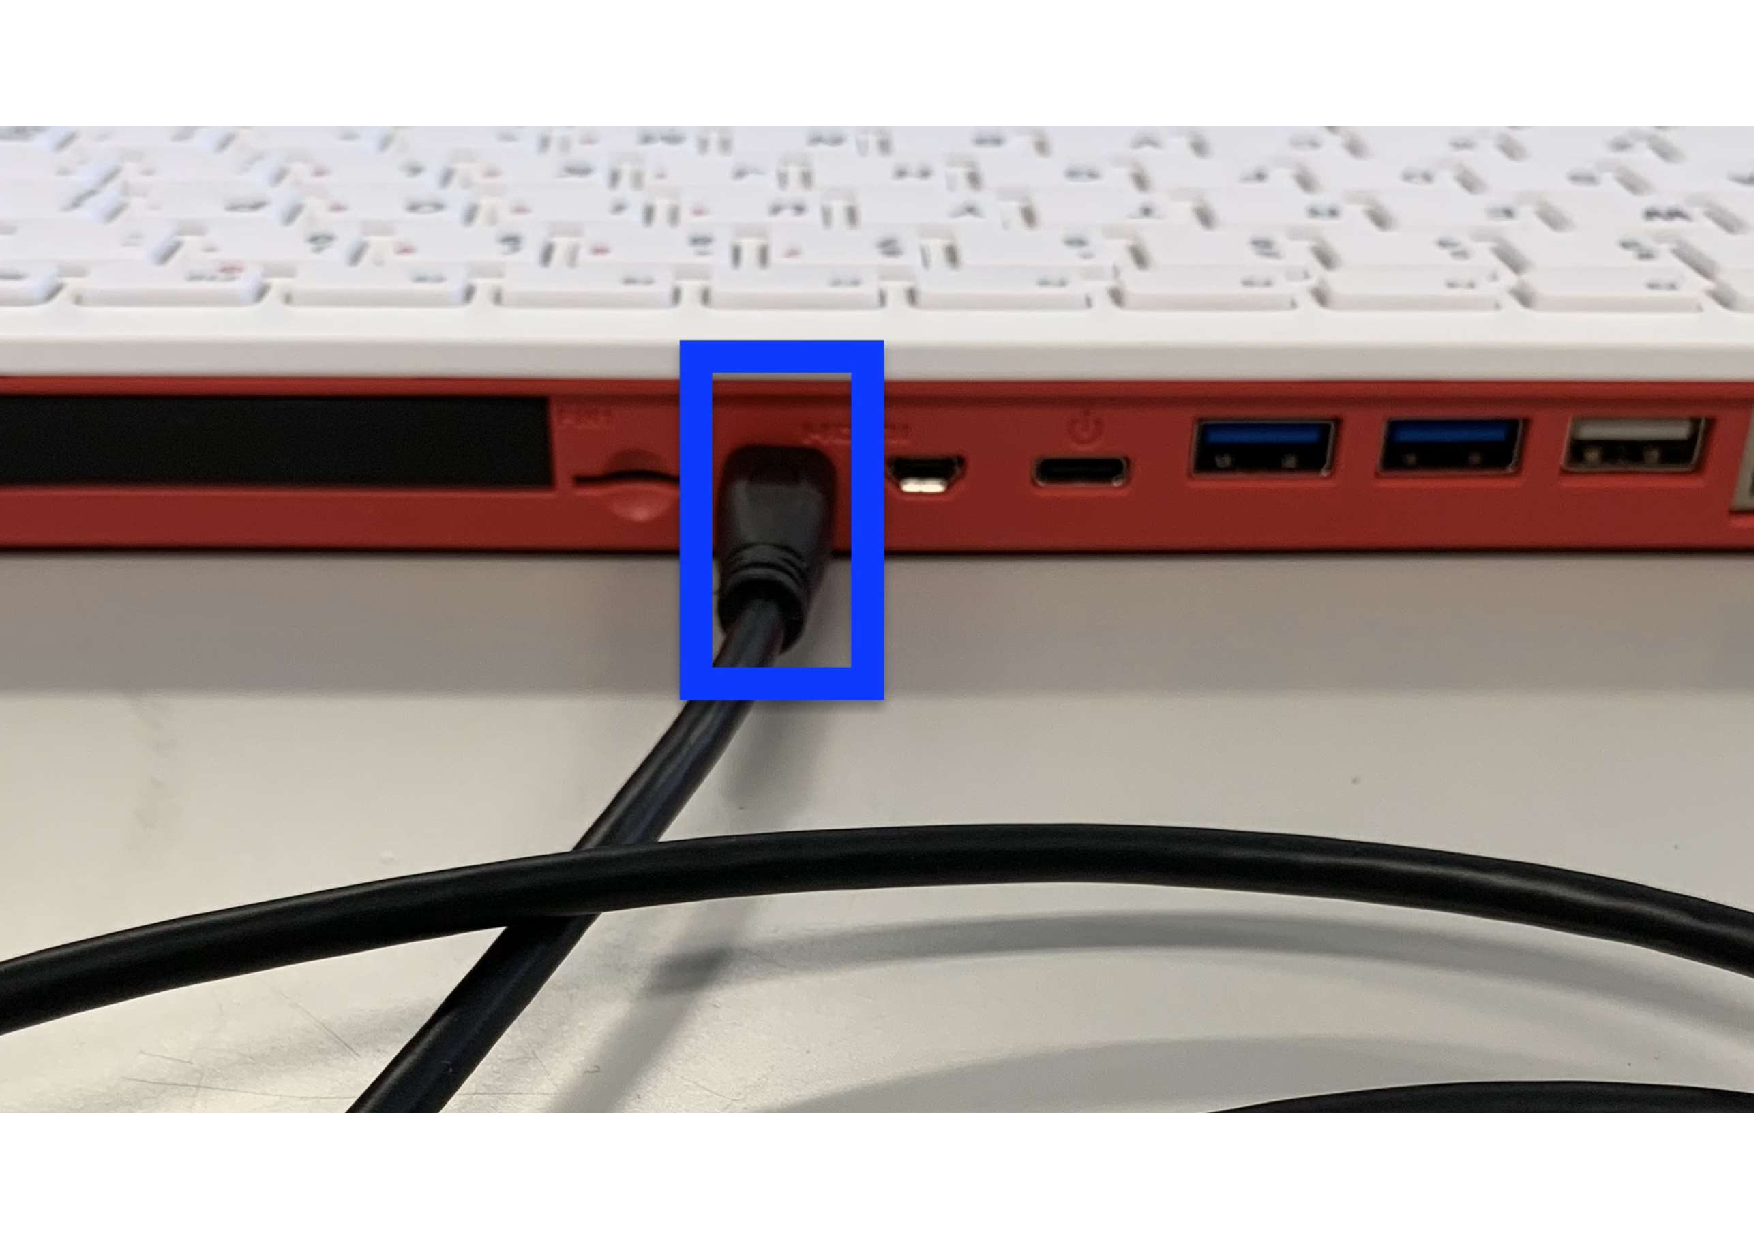
\includegraphics[width=5.519cm,height=3.471cm]{figure222023.pdf}
                      \newline
                      Figure {\refstepcounter{Figure}\theFigure\label{seq:refFigure1}}:
                      ラズベリーパイHDMI接続}
                  \end{minipage}
                  \begin{minipage}{0.5\textwidth}
                    {\upshape
                      %[Warning: Image ignored] % Unhandled or unsupported graphics:
                      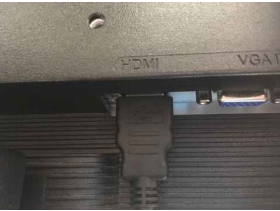
\includegraphics[width=5.519cm,height=3.471cm]{textbook-img016.png}
                      \newline
                      Figure {\refstepcounter{Figure}\theFigure\label{seq:refFigure2}}:
                      ディスプレイHDMI接続}
                  \end{minipage}
                \end{figure}

        \end{itemize}
  \item マウスとキーボードをつなぐ

        \begin{itemize}
          \item
                マウス、キーボードの先をラズベリーパイへ差し込みます。
        \end{itemize}
\end{enumerate}

\begin{figure}[h]
  \begin{minipage}{8.135cm}
    {\upshape
      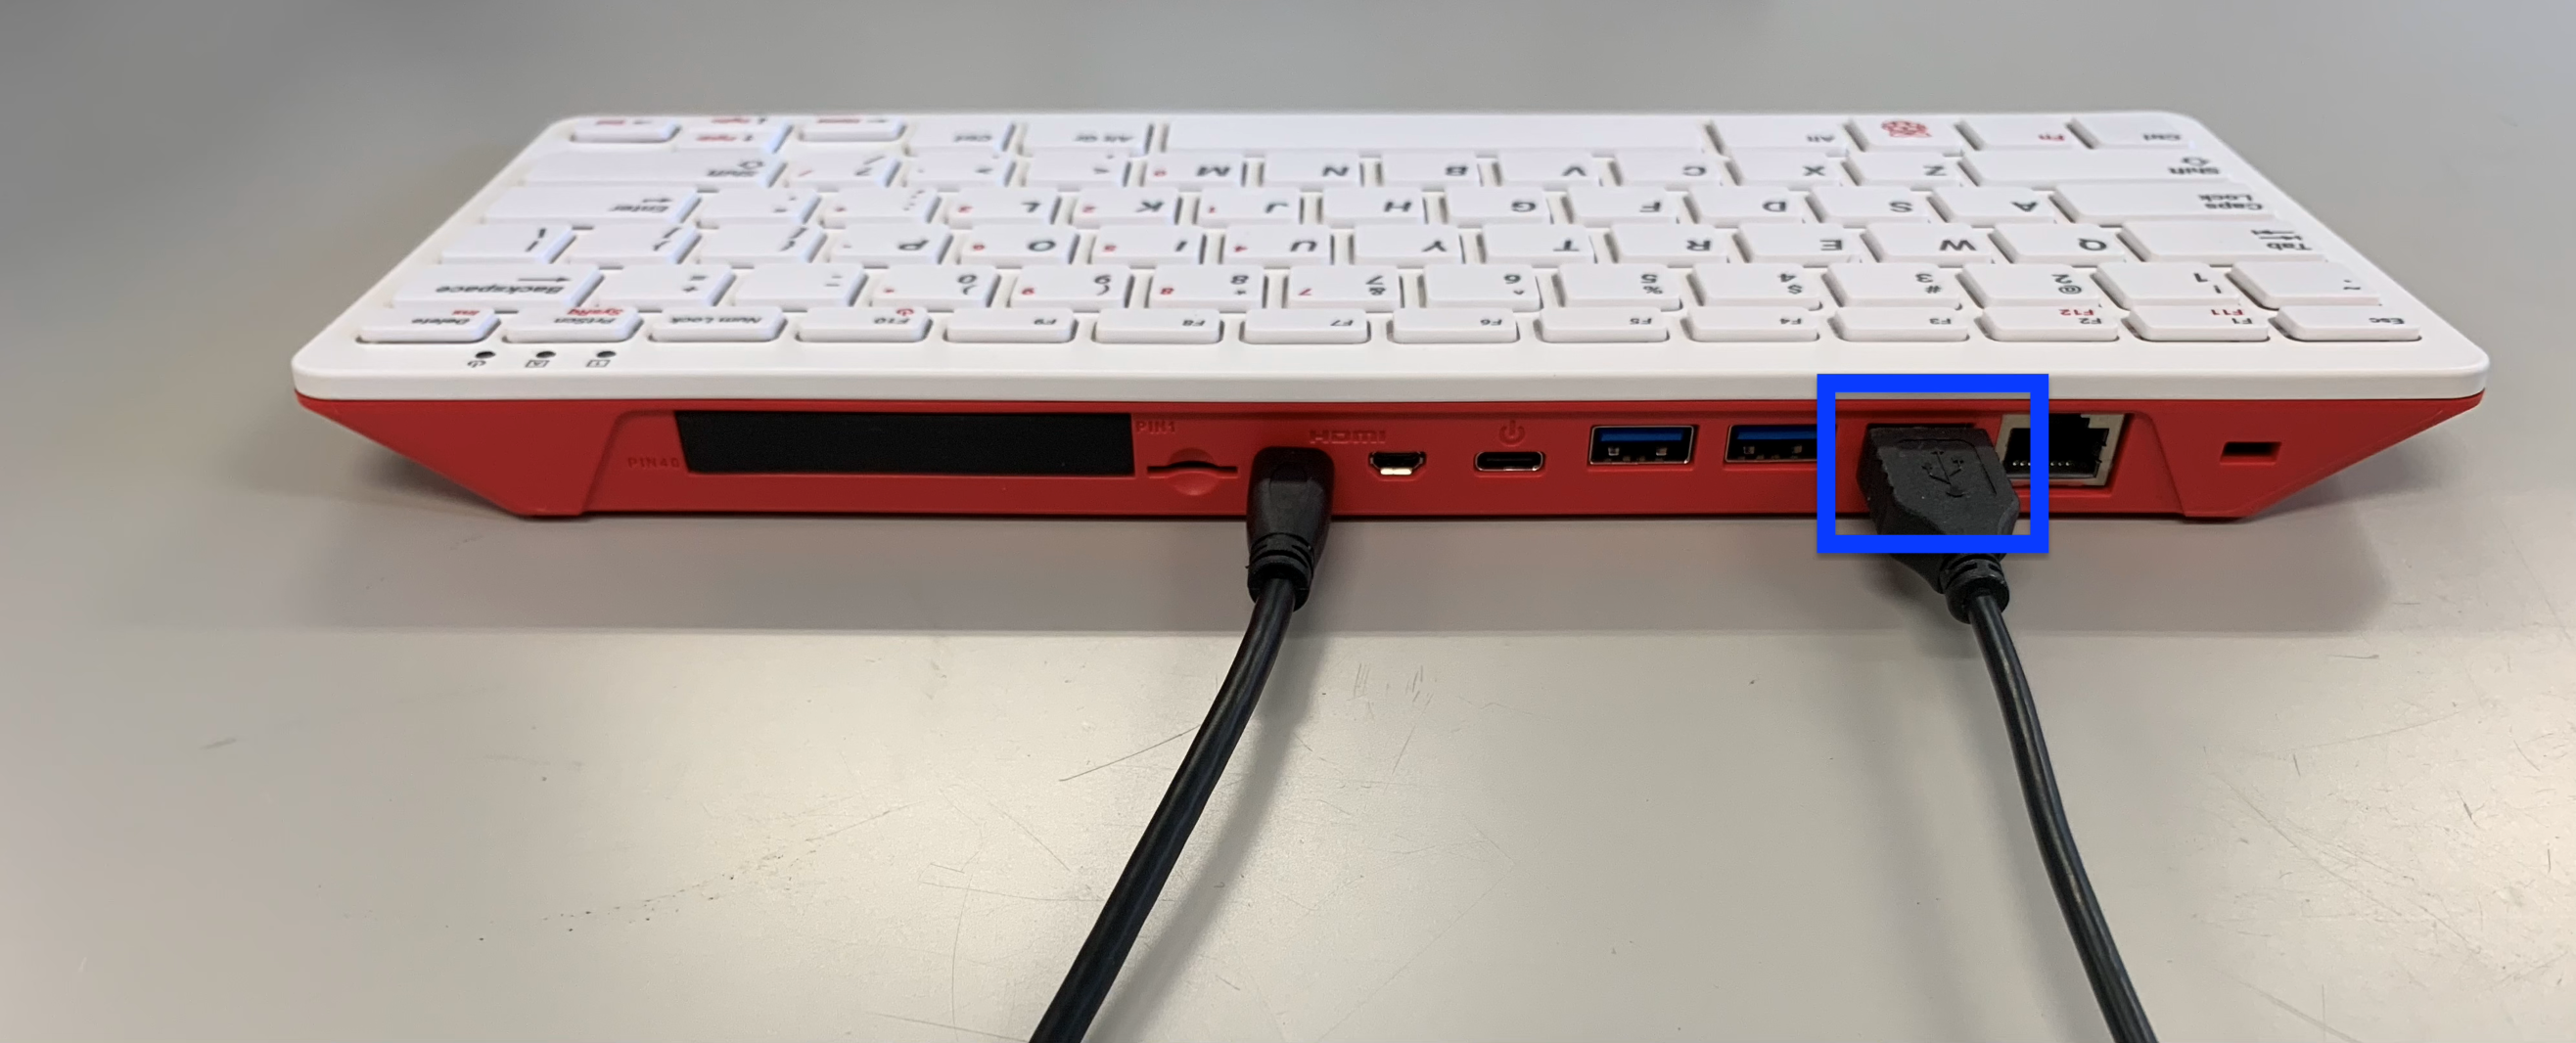
\includegraphics[width=8.135cm]{figure1.10-4.png}
      \newline
      Figure \stepcounter{Figure}{\theFigure}:
      マウス、キーボードの接続}
  \end{minipage}
\end{figure}
%\liststyleLxii
\setcounter{saveenum}{\value{enumi}}
\begin{enumerate}
  \setcounter{enumi}{\value{saveenum}}
  \clearpage
  \item
        microSD(マイクロエスディー)
        カードをいれる

        \begin{itemize}
          \item
                microSDカードをラズベリーパイ本体にさします。小さいのでなくさないように気をつけましょう。

                \begin{figure}[h]
                  \centering
                  \begin{minipage}{6.334cm}
                    {\upshape
                      \includegraphics[width=5.292cm,height=3.545cm]{figure1.10-5.png}
                      \newline
                      Figure \stepcounter{Figure}{\theFigure}: microSDカードのさしこみ}
                  \end{minipage}
                \end{figure}

                \bigskip
        \end{itemize}
  \item モニタのでんげんをいれる

        \begin{itemize}
          \item
                次にモニタのコンセントをさします。モニタのみぎはじのボタンをおします。でんげんが入ると青色にてんとうします。お家でやるときはでんげんのいれた後、入力きりかえが必要となる場合がありますので、説明書等を別途参照してください。


                \begin{figure}[h]
                  \centering
                  \begin{minipage}{6.172cm}
                    {\upshape
                      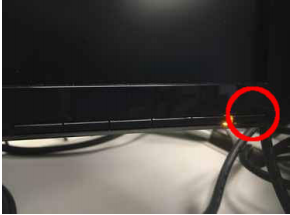
\includegraphics[width=6.318cm,height=4.685cm]{textbook-img019.png}
                      \newline
                      Figure \stepcounter{Figure}{\theFigure}:
                      モニタでんげんボタンの位置}
                  \end{minipage}
                \end{figure}
        \end{itemize}
  \item ラズベリーパイのでんげんをいれる

        \begin{itemize}
          \item
                最後にラズベリーパイのでんげんをいれます。Figure~\ref{seq:refFigure6}のようにラズベリーパイにでんげんケーブルをさしてコンセントへ接続します。緑色のランプがついてディスプレイにラズベリーが表示がされますFigure~\ref{seq:refFigure7}。
        \end{itemize}
        \begin{figure}
          \centering
          \begin{minipage}{5.228cm}
            {\upshape
              \includegraphics[width=4.613cm,height=3.856cm]{textbook-img020-2023.png}
              \newline
              Figure {\refstepcounter{Figure}\theFigure\label{seq:refFigure6}}:
              ラズベリーパイでんげん接続}
          \end{minipage}
          \begin{minipage}{5.371cm}
            {\upshape
              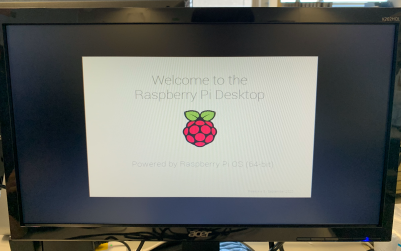
\includegraphics[width=4.782cm,height=3.919cm]{textbook-img0212023.png}
              \newline
              Figure {\refstepcounter{Figure}\theFigure\label{seq:refFigure7}}:
              ラズベリーパイ起動中}
          \end{minipage}
        \end{figure}
  \item インターネットに接続\\
        \ \ まずは画面右上のほうにあるWi-Fiのアイコンをクリックします。Figure~\ref{seq:refFigure10}の赤わくで囲われています。クリックするとFigure~\ref{seq:refFigure9}のようにWi-Fiのいちらんが出てきます。接続するアクセスポイントを選びます。

\end{enumerate}


\begin{figure}[h]
  \centering
  \begin{minipage}{6.597cm}
    {\upshape
      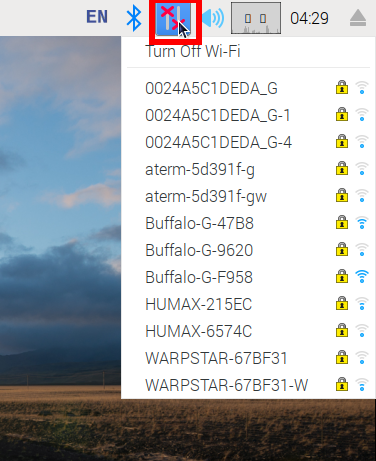
\includegraphics[width=4.068cm,height=4.987cm]{textbook-img024.png}
      \newline
      Figure {\refstepcounter{Figure}\theFigure\label{seq:refFigure10}}: Wi-Fi接続メニュー}
  \end{minipage}
  \begin{minipage}{5.957cm}
    {\upshape
      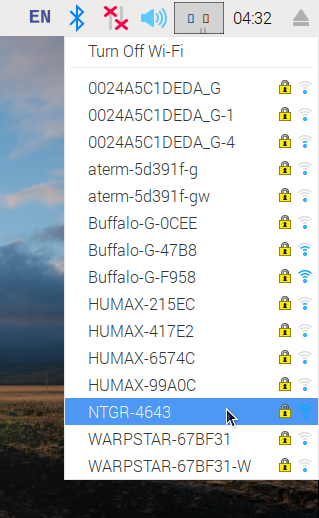
\includegraphics[width=3.427cm,height=4.738cm]{textbook-img023.png}
      \newline
      Figure {\refstepcounter{Figure}\theFigure\label{seq:refFigure9}}: SSIDいちらん}
  \end{minipage}
\end{figure}
にんしょうが必要なアクセスポイントの場合は、パスワードの入力を求められます。赤わくの中にパスワードを入力してOKを押します。

\begin{figure}
  \centering
  \begin{minipage}{7.712cm}
    {\upshape
      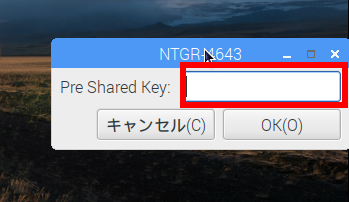
\includegraphics[width=7.712cm,height=3.888cm]{textbook-img026.png}
      \newline
      Figure \stepcounter{Figure}{\theFigure}: パスワード入力画面}
  \end{minipage}
  \begin{minipage}{7.241cm}
    {\upshape
      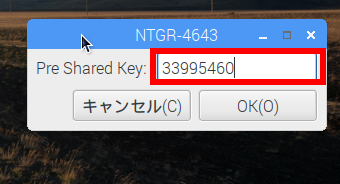
\includegraphics[width=5.577cm,height=3.228cm]{textbook-img025.png}
      \newline
      Figure \stepcounter{Figure}{\theFigure}: パスワード入力画面}
  \end{minipage}
\end{figure}
問題なく接続ができれば、Wi-FiのアイコンがFigure~\ref{seq:refFigure13}のようになります。これで接続は完了です。お家でやるときは、Wi-Fiのルーター等の説明書等を参照してください。

\begin{figure}
  \centering
  \begin{minipage}{7.334cm}
    {\upshape
      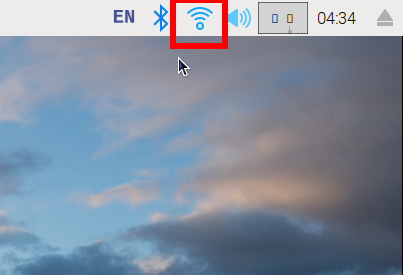
\includegraphics[width=5.708cm,height=3.895cm]{textbook-img027.png}
      \newline
      Figure {\refstepcounter{Figure}\theFigure\label{seq:refFigure13}}:
      接続後のアイコン}
  \end{minipage}
\end{figure}
\clearpage
\end{document}